\documentclass[11pt]{article}

\usepackage[margin=1in, a4paper]{geometry}

\usepackage[utf8]{inputenc}

\usepackage{setspace}  % set spacing

\setstretch{1.25}  %stretch line space to multiple x

\usepackage[dvipsnames,table, xcdraw]{xcolor}
% If you use beamer only pass "xcolor=table" option, i.e. \documentclass[xcolor=table]{beamer}

\usepackage{shadowtext}

\usepackage{indentfirst} % indent the first paragraph of each section

\usepackage{float} %determine the position of figures in the document

\usepackage{tabularx} % extra features for tabular environment

\usepackage{amsmath, amsfonts, amssymb}  % improve math presentation

\usepackage{blkarray, bigstrut}

\usepackage{makecell}

\usepackage{mathtools}
\DeclarePairedDelimiter\ceil{\lceil}{\rceil}
\DeclarePairedDelimiter\floor{\lfloor}{\rfloor}



%++++++++++++++++++++++++++++++++++++++++++++++++++++++++++++++++

\usepackage{graphicx} % takes care of graphic including machinery

\graphicspath{ {../../logos/} }

%++++++++++++++++++++++++++++++++++++++++++++++++++++++++++++++++



\usepackage{caption}

\usepackage{subcaption}

\usepackage{tikz}

\usepackage{lipsum,lmodern}

\usepackage[most]{tcolorbox}

\usetikzlibrary{trees}  %add binary trees

\usetikzlibrary {positioning}

\usepackage[final]{hyperref} % adds hyper links inside the generated pdf file

\hypersetup{
	colorlinks=true,       % false: boxed links; true: colored links
	linkcolor=blue,        % color of internal links
	citecolor=blue,        % color of links to bibliography
	filecolor=magenta,     % color of file links
	urlcolor=blue         
}

\usepackage{blindtext}

\usepackage{dirtytalk} %quotation marks


%********************************

%Bibliography

\usepackage[backend=biber,  style=alphabetic,  sorting=ynt]{biblatex}

\addbibresource{../../Mybib.bib}


%********************************


\usepackage{fancyhdr}

\pagestyle{fancy}

\fancyhf{}

\lhead{\footnotesize {Math notes: Proof of CLT by mgf} }
\rhead{\footnotesize { } }
\cfoot{- \thepage \ -}

\title{\vspace{-90pt} 


%**************************************************

% Title Part
\textbf  {Peer-graded Assignment} }
\author{Cui, Xiaolong(Larry)}
\date{\today}


%*************************************************

\begin{document}

%\maketitle

\thispagestyle{plain}

%*************************************************

\begin{figure}[H] %[!tbp]
  \begin{subfigure}{0.3\textwidth}
    
\includegraphics[width=\textwidth]{uol}
    %\caption{Flower one.}
    %\label{fig:f1}
  \end{subfigure}
  \hfill
  \begin{subfigure}{0.3\textwidth}
    \includegraphics[width=\textwidth]{goldsmiths}
    %\caption{Flower two.}
    %\label{fig:f2}
  \end{subfigure}
  %\caption{My flowers.}
\end{figure}

%****************************************************

\begin{flushright}

\footnotesize {Sept. 21st,  2021}
\end{flushright}

\begin{center}
\textbf{A Weak Proof of the Central Limit Theorem \\
with Moment Generating Function} \\
\footnotesize {Study Notes $ | $ Written by Larry Cui}
\end{center}

%***************************************************

%\begin{abstract}
%\end{abstract}


%***************************************************

\setcounter{figure}{0}

\vspace{10pt}


Central Limit Theorem (CLT) is one of the two most important theorems in statistics (the other is the Large Number Theorem).  In this note,  the theorem of moment generating function (\textit {mgf}) is used to prove the CLT without proving the mgf theorem itself.  So we call this a weak proof.  Notice that mgf may not always exist for all functions,  so sometimes people use characteristic function instead to prove CLT.



\section {\large Moment Generating Function}

\begin{tcolorbox}[
	enhanced, 
	width=\textwidth, 
	%center upper,
	fontupper=\normalsize,% \bfseries,
	drop fuzzy shadow southwest,
	boxrule=0.4pt,
	sharp corners,
	colframe=yellow!80!black,
	colback=yellow!10]
	
\textbf{\color{RoyalBlue} Definition} 

\qquad Let $W$ be a random variable.  The moment generating function (mgf) for $W$ is denoted $M_W (t)$ and given by
\[ 
M_W (t) = E(e^{tW}) =  \left\{
\begin{array}{ll}
    \displaystyle  \sum _{ \text{all $k$} } e^{tW} p_W(k)  & \text{if $W$ is discrete} \\
    \hspace{5pt} \\
    \displaystyle \int _{-\infty} ^{\infty} e^{tW} f_W (w) \, dw  & \text{if $W$ is continuous} \\
\end{array} 
\right. 
\]
at all values of $t$ for which the expected value exists.

\end{tcolorbox}


In short, mgf is the expected value of $e^{tW}$ for the generating function that has the pdf of $p_W(k)$ or $f_W (w)$,  in discrete or continuous way,  respectively.   Sometimes, due to the property of the function,  the expected value may go to infinity,  and we say under such situation the mgf does not exist.

An illustration of mgf for \textbf {binomial random variable} $X$ with pdf:
$$
p_X (k) = \binom{n}{k} p^k (1-p)^{n-k}
$$
is
$$
\begin{aligned}
M_X (t) = E(e^{tx})
	&= \sum ^n _{k=0} e^{tk} \binom{n}{k} p^k (1-p)^{n-k} \\
	&= \sum ^n _{k=0} \binom{n}{k} (pe^t)^k (1-p)^{n-k} \\
	&= (1-p + pe^t) ^n \\
\end{aligned}
$$

Another example is for \textbf {Poisson random variable}:
$$
p_X (k) = \frac{e^{-\lambda} \lambda ^k}{k!}
$$
and
$$
\begin{aligned}
M_X(t) = E(e^{tx})
	&= \sum _{k=0} ^ \infty e^{tk} \frac {e^{-\lambda} \lambda ^k} {k!} \\
	&= e^{-\lambda} \sum _{k=0} ^ \infty \frac{ (e^t \lambda)^k} {k!}\\
	&= e^{-\lambda} e^{\lambda e^t} \\
	&= e^{-\lambda + \lambda e^t} \\
\end{aligned}
$$




\section {\large Some Important Features of mgf}

\begin{tcolorbox}[
	enhanced, 
	width=\textwidth, 
	%center upper,
	fontupper=\normalsize,% \bfseries,
	drop fuzzy shadow southwest,
	boxrule=0.4pt,
	sharp corners,
	colframe=yellow!80!black,
	colback=yellow!10]
	
\textbf{\color{RoyalBlue} mgf Theorem} 

\qquad Suppose that $W1$ and $W2$ are random variables for which $M_{W_1} (t) = M_{W_2} (t)$ for some interval of $t$'s containing $0$.  Then $f_{W_1} (w) = f_{W_2} (w)$.

\end{tcolorbox}

We will leave the proof of this theorem to further notes,  but use this result directly to prove CLT. 

That being said,  we can still get some feeling about this theorem by intuition,  for we know that
$$ M ^{(0)} _W (0) = \int e^{0w} f_W (w) \, dw = \int f_W (w) \, dw = 1$$ and
$$ M ^{(1)} _W (0) = \int w e^{0w} f_W (w) \, dw =  \int w  f_W (w) \, dw = E(W) $$ and
$$ M ^{(2)} _W (0) = \int w^2 e^{0w} f_W (w) \, dw = \int w^2  f_W (w) \, dw = E(W^2) $$
$$ \dots $$
$$ M ^{(n)} _W (0) = \int w^n e^{0w} f_W (w) \, dw = \int w^n  f_W (w) \, dw = E(W^n) $$

So we know that if two function's mgf are the same,  then their expected values for random variables itself and higher orders are also the same.  And since expected value,  variance and other properties of a function can be represented by its mgf,  we can almost tell that the two functions will behave same.   The missing piece of this intuitive understanding is obvious,  however: it does not rule out the possibility that why two different functions cannot generate the same mgf. 

We move on to the next two important properties of mgf.

\begin{tcolorbox}[
	enhanced, 
	width=\textwidth, 
	%center upper,
	fontupper=\normalsize,% \bfseries,
	drop fuzzy shadow southwest,
	boxrule=0.4pt,
	sharp corners,
	colframe=yellow!80!black,
	colback=yellow!10]
	
\textbf{\color{RoyalBlue} lemma a.}  \ \ Let $W$ be a random variable with mgf $M_W (t)$.  Let $V=aW + b$.  Then
$$
M_V (t) = e^{bt} M_W (at)
$$

\end{tcolorbox}

\textbf{Proof}:  we prove the lemma for continuous function,  the discrete function is the same.
$$
\begin{aligned}
M_V (t)
	&= \int e^{t (aW +b)} f_V (v) \, dv \\
	&= \int e^{t (aW +b)} \frac{1}{|a|} f_W (w) a \, dw \\
	&= \int e^{t (aW +b)} f_W (w)  \, dw \\
	&= e^{bt} \int e^{atW} f_W (w)  \, dw \\
	&= e^{bt} M_W (at) \\
\end{aligned}
$$

\begin{tcolorbox}[
	enhanced, 
	width=\textwidth, 
	%center upper,
	fontupper=\normalsize,% \bfseries,
	drop fuzzy shadow southwest,
	boxrule=0.4pt,
	sharp corners,
	colframe=yellow!80!black,
	colback=yellow!10]
	
\textbf{\color{RoyalBlue} lemma b.}  Let $W_1, W_2,  \dots , W_n$ be independent random variables with mgfs $M_{W_1} (t),  M_{W_2} (t),  \dots,  M_{W_n} (t)$,  respectively.  Let $W = W_1 + W_2 + \cdots + W_n$.  Then
$$
M_W (t) = M_{W_1} (t) \cdot M_{W_2} (t) \cdots M_{W_n} (t)
$$

\end{tcolorbox}

\textbf{Proof}: In order to prove lemma b.,  we only need to prove that $ M_W(t) = M_{W_1} (t) \cdot M_{W_2} (t)$ if  $W = W_1 + W_2 $.  Because $W_1$ and $W_2$ are independent variables,  we have pdf and cdf for $W$: 
\begin{center}
$f_W (w) = f_{W_1} (w_1) f_{W_2} (w_2) $ \hspace{15pt}  and  \hspace{15pt} $F_W(w) = \displaystyle \iint  f_{W_1} (w_1) f_{W_2} (w_2) \, dw_1 \,dw_2 $
\end{center}
and mgf for $W$: 
$$
\begin{aligned}
M_W (t) = E(e^{t(W_1 + W_2)}) 
	&= \iint e^{t(W_1 + W_2)}  f_{W_1} (w_1) f_{W_2} (w_2) \, dw_1 \,dw_2 \\
	&= \int e^{tW_1}  f_{W_1} (w_1) \, dw_1 \cdot \int e^{tW_2}  f_{W_2} (w_2) \, dw_2 \\ 
	&= M_{W_1} (t) \cdot M_{W_2} (t) \\
\end{aligned}
$$



\section {\large Normal Distribution Function}

\begin{tcolorbox}[
	enhanced, 
	width=\textwidth, 
	%center upper,
	fontupper=\normalsize,% \bfseries,
	drop fuzzy shadow southwest,
	boxrule=0.4pt,
	sharp corners,
	colframe=yellow!80!black,
	colback=yellow!10]
	
\textbf{\color{RoyalBlue} pdf of a normal distribution} 
\begin{center}
$\displaystyle f_Y(y) = \frac{1}{\sqrt{2\pi} \sigma} \exp \left[ - \frac{1}{2} \left( \frac{y - \mu }{\sigma} \right) ^ 2 \right]$ \hspace{5pt},  \hspace{5pt} $-\infty < y < \infty$
\end{center}

\end{tcolorbox}

Depending on the values of $\mu$ and $\sigma$,  the pdf curve can take different shapes.  When $\mu = 0$ and $\sigma = 1$,  the normal distribution becomes $\displaystyle  \frac{1}{\sqrt{2\pi}} \cdot e^{-t^2/2} $ and is called \textbf{standard}. 

\begin{figure}[H] %[!tbp]
	\centering
 	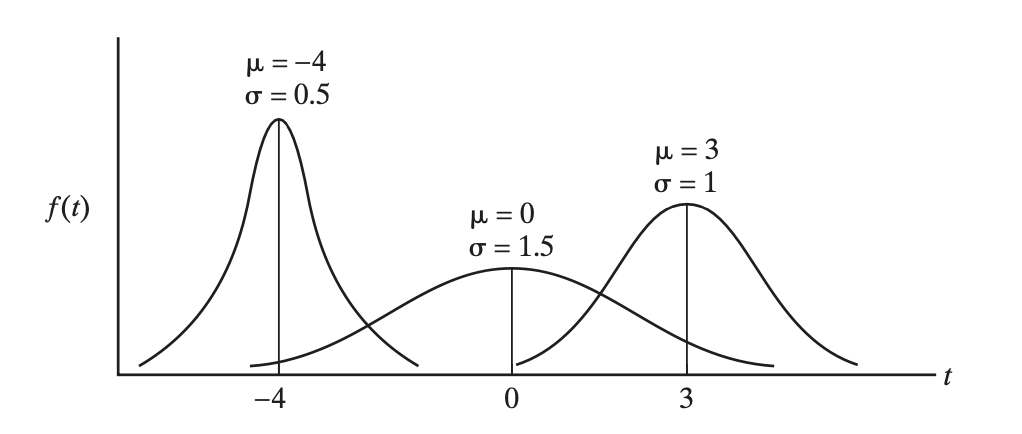
\includegraphics[width=0.7\textwidth]{normal_shapes}
 	\caption{normal curves with different $\mu$ and $\sigma$}
  	\label{fig:}
\end{figure}

The adding up of pdf $f_Y(y)$ to $1$ needs some polar coordinates integral techniques.  But first of all,  let's see if we can simplify this function for the integration purpose.  We can tell from Figure 1 above that $\mu$ determine the location of the curve,  but has nothing to do with the shape itself.  So let $\mu = 0$ won't lose generosity to the calculation while gives us a huge convenience.   

\textbf {Proof}:  the basic idea is that we square the cdf of $f_Y(y)$,  if the result equals 1,  then cdf must be 1.  We re-write the pdf as follows (deleting the $\mu$ part):
$$ 
f_Y(y) = \frac{1}{\sqrt{2\pi} \sigma} \exp \left[ - \frac{1}{2} \left( \frac{y}{\sigma} \right) ^ 2 \right]
$$

If we square the cdf of a function,  the mathematical meaning is to find the joint density in an $xy$-plane,  where $x$ and $y$ axes have the same pdf.
$$
\text {cdf} ^2 = \frac{1}{\sqrt{2\pi} \sigma} \int _{-\infty} ^\infty e^{- \frac{x^2}{2 \sigma^2}} \, dx \cdot \frac{1}{\sqrt{2\pi} \sigma} \int _{-\infty} ^\infty e^{- \frac{y^2}{2 \sigma^2}} \, dy = \frac{1}{2\pi \sigma^2} \int _{-\infty} ^\infty \int _{-\infty} ^\infty e^{- \frac{1}{2 \sigma^2} (x^2 + y^2)} \, dx \,dy
$$

Let $x=r \cos \theta$ and $y= r \sin \theta$,  then $\,dx \,dy = r \,dr \, d\theta$,  and 
$$
\begin{aligned}
\frac{1}{2\pi \sigma^2} \int _{-\infty} ^\infty \int _{-\infty} ^\infty e^{- \frac{1}{2 \sigma^2} (x^2 + y^2)} \, dx \,dy
	&= \frac{1}{2\pi \sigma^2} \int _0 ^{2\pi} \int _0 ^\infty e^{- \frac{r^2}{2 \sigma^2}} r \, dr \,d\theta \\
	&= \frac{1}{2\pi \sigma^2} \int _0 ^\infty e^{- \frac{r^2}{2 \sigma^2}} r \, dr \int _0 ^{2\pi} \,d\theta \\
	&= \frac{1}{2\pi \sigma^2} \cdot \sigma^2 \cdot 2\pi \\
	&= 1\\
\end{aligned}
$$


\begin{tcolorbox}[
	enhanced, 
	width=\textwidth, 
	%center upper,
	fontupper=\normalsize,% \bfseries,
	drop fuzzy shadow southwest,
	boxrule=0.4pt,
	sharp corners,
	colframe=yellow!80!black,
	colback=yellow!10]
	
\textbf{\color{RoyalBlue} mgf of a normal distribution} 
$$
M_Y (t) = \exp \left[ \mu t + \frac{\sigma^2 t^2}{2} \right]
$$
and 
\begin{center}
$M_Y(t) = e^{\frac{t^2}{2}}$ \hspace{5pt} when $\mu = 0$ and $\sigma =1$
\end{center}


\end{tcolorbox}


\textbf{Calculating process of $M_Y(t)$}:
\[
\begin{aligned}
M_Y(t) = E(e^{ty})
	&= \frac{1}{\sqrt{2\pi} \sigma} \int _{-\infty} ^\infty e^{ty} \exp \left[ -\frac{1}{2} \left( \frac{y - \mu}{\sigma} \right) ^2 \right] \, dy \\
	&=\frac{1}{\sqrt{2\pi} \sigma} \int _{-\infty} ^\infty  \exp \left[ -\frac{y^2 - 2\mu y + \mu^2 - 2 \sigma^2 ty } {2 \sigma^2} \right] \, dy \\ \\
\end{aligned}
\]

Using a little technique,  we can re-arrange the terms in the brackets as
$$ y^2 - (2\mu + 2 \sigma^2 t)y + (\mu + \sigma^2t) ^2 -(\mu + \sigma^2t) ^2  + \mu^2 $$
$$ = [y - (\mu + \sigma^2 t)] ^2 - \sigma^4 t^2 + 2 \mu t \sigma^2 $$

The last two terms involves no $y$,  so can be moved out of the integral
$$
M_Y(t) = \exp \left( \mu t + \frac{\sigma^2 t^2}{2} \right)  \underbrace{ \frac{1}{\sqrt{2\pi} \sigma}  \int _{-\infty} ^\infty \exp \left[ - \frac{1}{2}\left[ \frac{y - (\mu + t \sigma^2)}{\sigma} \right]^2 \right] \, dy } _\textrm{equals 1}
$$
The latter part is still the cdf of a normal curve with $\mu' = (\mu + t\sigma^2)$,  so the mgf is shortened to the first part of the equation. 




\section {\large Central Limit Theorem}


\begin{tcolorbox}[
	enhanced, 
	width=\textwidth, 
	%center upper,
	fontupper=\normalsize,% \bfseries,
	drop fuzzy shadow southwest,
	boxrule=0.4pt,
	sharp corners,
	colframe=yellow!80!black,
	colback=yellow!10]
	
\textbf{\color{RoyalBlue} CLT:} \ \ \ \ Let $Y_1,Y_2, \dots, Y_n$ be independent and identically distributed random variables with $E(Y_i) = \mu$ and $ Var (Y_i) = \sigma^2$ (both $< \infty$).  Define
\begin{center}
$ \displaystyle U_n = \frac{\displaystyle \sum ^n _{i=1} Y_i - n \mu}{\sigma \sqrt{n} } = \frac{ {\overline {Y} } - \mu}{\sigma / \sqrt{n} }$  \hspace{10pt} where $\overline {Y} = \displaystyle \frac{1}{n} \sum _{i=1} ^n Y_i$
\end{center}
Then the distribution function of $U_n$ converges to the standard normal distribution function as $n \to \infty$.  That is,  for all $u$ ($u$ is the value that variable $U_n$ takes)
$$
\lim _{n \to \infty} P (U_n \leqslant u) = \int _{-\infty} ^u \frac{1}{\sqrt{2 \pi} } e^{-\frac{t^2}{2}} \, dt
$$

\end{tcolorbox}


The ordinary language interpretation of the CLT is that,  no matter what the pdf is for the original function $f_Y(y)$,  the sum or arithmetic average of $Y_i$,  when $i$ is big enough, \footnote{By convention,  $i>30$ will give us a pretty decent approximation.}  tends to match the normal distribution.    

\textbf{Why $U_n$?}

$U_n$ has a strange looking compared to sum or average of $Y_i$.  But if the sum or average of $Y_i$ has already followed the normal distribution,  why should we construct $U_n$ in such an awkward looking way to bring out the CLT?   The reason is for \textbf{standardization}.  \footnote{Actually,  we can never know the exact values of $\mu$ and $\sigma$ of the total population.  But how to find approximated values are another topic.} Let's presume $Y_i$ follows normal distribution for the time being,  then the sum or average would have an expected value and variance as
$$
E\left( \sum ^n _{i=1} Y_i  \right) = E(Y_1) + E(Y_2) + \cdots + E(Y_n) = n\mu
$$
and \cite[p.~188]{larsen2012introduction}  
$$
V \left( \sum ^n _{i=1} Y_i  \right) = V(Y_1) + V(Y_2) + \cdots + V(Y_n) = n\sigma^2
$$
or
$$
E(\overline {Y}) = \frac{1}{n} [ E(Y_1) + E(Y_2) + \cdots + E(Y_n) ] = \mu
$$
and
$$
V( \overline {Y} ) = \frac{1}{n^2} [ V(Y_1) + V(Y_2) + \cdots + V(Y_n) ]  = \frac{\sigma^2}{n}
$$

Conclusion: variable $U_n$ is constructed in such a way that it always has $\mu = 0$ and $\sigma = 1$,  a standard form easy for analysis and calculation, where simplified normal distribution probability $e^{-t^2/2}$ are available everywhere. 

Before proving the theorem,  we also need a lemma about the mgf:

\begin{tcolorbox}[
	enhanced, 
	width=\textwidth, 
	%center upper,
	fontupper=\normalsize,% \bfseries,
	drop fuzzy shadow southwest,
	boxrule=0.4pt,
	sharp corners,
	colframe=yellow!80!black,
	colback=yellow!10]
	
\textbf{\color{RoyalBlue} lemma c.} \ \ \ \ mgf can by approximated by polynomial.  If we use Taylor's Theorem (here Maclaurin series,  specifically),  that 
$$
M(t) = M(0) + M'(0)t + M''(0)\frac{t^2}{2!} + \cdots + M^{(n)}(0)\frac{ t^n}{n!} + M^{(n+1)}(\xi) \frac{t^{n+1}}{(n+1)!}
$$
where $0<\xi<t$.
\end{tcolorbox}


\textbf{Proof of CLT}:

\hspace{5pt}

Because $ \displaystyle U_n = \frac{1}{\sqrt{n}} \frac{ \sum ^n _{i=1} Y_i - n \mu}{\sigma}$ ,  if let $\displaystyle Z_i =  \frac{Y_i - \mu}{\sigma}$, we can write $U_n$ as:
$$
U_n = \frac{1}{\sqrt{n}} \sum ^n _{i=1} Z_i
$$

Since we know from the condition of the theorem that $E(Y_i) = \mu$ and $ Var (Y_i) = \sigma^2$,  then
\begin{center}
$E(Z_i) = 0$ \hspace{10pt} and \hspace{10pt} $V(Z_i) = 1$
\end{center}

$Z_i$ is based on $Y_i$,  which in turn comes from the same population,  so each and every $Z_i$ must have the same pdf and mgf.  Now we can re-write $M_{U_n} (t)$ as
\[
\begin{aligned}
M_{U_n} (t)
	&= M_{\frac{1}{\sqrt{n} } \sum Z_i} (t) \\
	&= M_{\sum Z_i} \left( \frac{t}{\sqrt{n}} \right) \\
	&= \left[ M_{Z_1} \left(  \frac{t}{\sqrt{n}} \right) \right] ^n \qquad  \text{\color{RoyalBlue} by lemma b.} \\
\end{aligned}
\]

but $M_{Z_1} (t)$ can be written as a polynomial series by lemma c,
\begin{center}
$ M_{Z_1} (t) = M_{Z_1} (0) + M'_{Z_1} (0) t + M''_{Z_1} (\xi) \frac{t^2}{2} ,  \qquad \text{where} \ \ 0<\xi<t$
\end{center}

and because $M_{Z_1} (0) = E(e^{0Z_1}) = E(1) = 1$,  and $M' _{Z_1} (0) = E(Z_1) = 0$,  the above series reduces to
\begin{center}
$M_{Z_1} (t) = 1 + \displaystyle \frac {M''_{Z_1} (\xi)} {2} t^2$,  \qquad where \ \ $0<\xi<t$
\end{center}
as $t$ is dummy variable here,  it can be replaced by any other variables.  If we replace it with $t/ \sqrt{n}$,  then
$$
M_{Z_1} \left(  \frac{t}{\sqrt{n}} \right) = 1 + \frac {M''_{Z_1} (\xi')} {2} \left( \frac{t}{\sqrt{n}} \right)^2  \qquad \text{where} \ \ 0<\xi'< \frac{t}{\sqrt{n}}
$$

Now we have an updated form for $M_{U_n} (t)$:
\[
\begin{aligned}
M_{U_n} (t)
	&= \left[ 1 + \frac {M''_{Z_1} (\xi')} {2} \left( \frac{t}{\sqrt{n}} \right)^2 \right] ^n \\
	&= \left[ 1 + \frac {M''_{Z_1} (\xi') t^2 /2} {n} \right] ^n \\
\end{aligned}
\]
Notice that as $n \to \infty$, $\xi' \to 0$,  so $M'' _{Z_1} (\xi') \to M'' _{Z_1} (0) $,  and
$$
M'' _{Z_1} (0) = E(Z_1^2) = V(Z_1) + E(Z_1)^2 = 1
$$
further reduce $M_{U_n} (t)$ to
$$
M_{U_n} (t) = \left[ 1 + \frac {t^2 /2} {n} \right] ^n  \qquad \text{where} \ \ n \to \infty
$$
which is a familiar form for $e$ to the power of anything above $n$,  and here comes our conclusion: 
$$
M_{U_n} (t) = e^{\frac{t^2}{2}}
$$

This is exactly the mgf of a normal distribution function with $\mu=0$ and $\sigma=1$.  Also be noted that we didn't use pdf of the generating function to reach the mgf,  which is in line with the CLT assertion that it applies to all functions no matter what pdf it is.  So the proof.













%++++++++++++++++++++++++++++++++++++++++

\clearpage

\printbibliography [title={Reference}]


%***********************************

\end{document}
